\section{CPU Architecture}

Hazard5 is a 32-bit processor based on the RISC-V instruction set architecture. It accesses the system through a single AMBA 3 AHB-Lite master port. Those familiar with the textbook 5-stage RISC pipeline will find Hazard5 mostly straightforward, but hopefully will still find some interesting tricks. We will use the following symbols to refer to the 5 stages:

\begin{itemize}
\item {\tt F}: fetch
\item {\tt D}: decode
\item {\tt X}: execute
\item {\tt M}: memory access (load/store)
\item {\tt W}: register writeback, fetch address generation
\end{itemize}


Hazard5 supports the RV32IC instruction set, whose encoding is variable-width. The C extension typically reduces instruction bandwidth by \textasciitilde 25\%, which helps to maintain performance when sharing bus access between fetch and load/store.

Branches are speculated, but there is currently no dynamic branch predictor. Instead, we use the static prediction scheme described in the RV ISA manual (based on sign of branch offset).

\subsection{Frontend}
\label{section:frontend}

\begin{figure}[!htb]
\centering
\caption{Hazard5 processor frontend, block diagram}
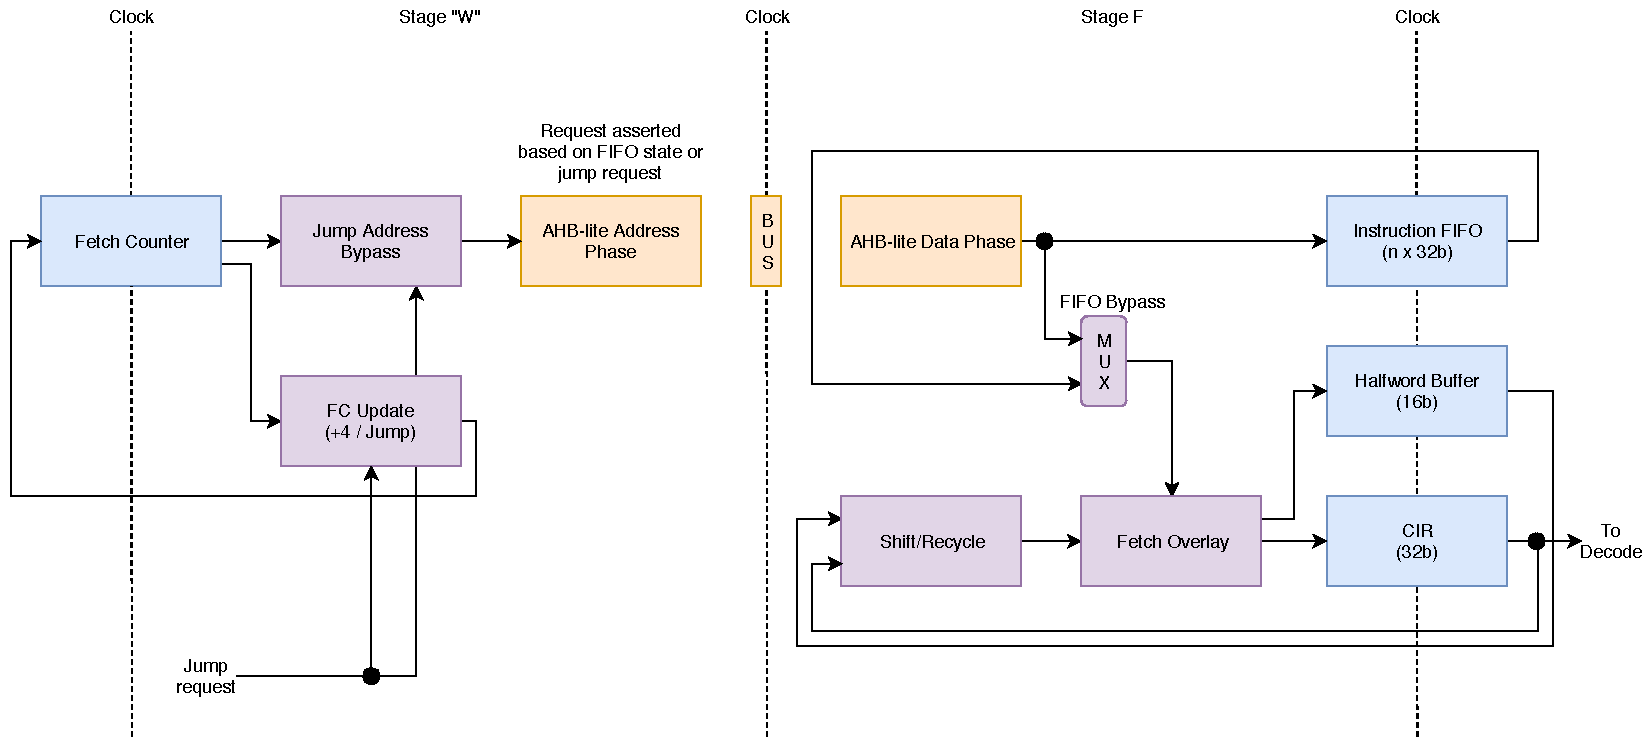
\includegraphics[width=0.9\textwidth]{diagrams/cpu_frontend.pdf}
\label{diagram:frontend}
\end{figure}

The frontend (figure \ref{diagram:frontend}) consists of stage {\tt F} and an additional stage which performs the AHB address phase, and can be considered part of {\tt W}. Its purpose is to feed {\tt D} with instructions, whilst meeting the following constraints:

\begin{itemize}
	\item No combinatorial path from AHB-Lite data phase to address phase (e.g. {\tt hready} $\to$ {\tt htrans})
	\item AHB-Lite compliant: no unaligned transfers, no deassertion or change of active requests
	\item Provide up to 32 bits of instruction data per clock in steady state, even if instructions are unaligned
	\item 0-cycle jump/flush to AHB address phase assertion (with minimal logic on this path)
	\item No performance penalty for unaligned jump to 16-bit instruction
	\item Attempt to maintain performance when competing with the load/store unit and AHB-Lite busmaster peers
\end{itemize}

The main source of complexity is that a RISC-V *C instruction stream is not naturally-aligned, i.e. instruction address modulo instruction size is not always zero. We spend gates here to optimise the common case of sequential execution, and to lessen the effects of fetch starvation due to load-store activity.

To meet these constraints, the frontend performs almost exclusively word accesses, which must be aligned. The only exception is a jump (or similar, e.g. mispredict recovery) to a non-word-aligned address. In this case, a halfword fetch from the target address is performed.

\subsubsection{Prefetch Queue}

The frontend queues up fresh instruction data which is waiting to be decoded. The pipelined nature of AHB-Lite means that the bus transfers run ahead of {\tt D} by at least two clocks, and the prefetch queue is able to buffer these in-flight transfers if {\tt D} stalls against a later pipe stage. The queue also decouples {\tt D}'s stall logic (which is a function of {\tt hready}) from the address phase request, and finally, the queue helps keep {\tt D} supplied with instructions while the busmaster is busy with load/stores from {\tt X}.

There are three parts to the queue:

\begin{itemize}
	\item A 32-bit FIFO. The depth is configurable, and can be as little as 1 word.
	\item A halfword buffer which may store the higher-addressed half of a recently-popped FIFO word
	\item The upper half of the current instruction register ({\tt CIR}), if the previous instruction was 16-bit
\end{itemize}

These three sources should service the majority of instruction fetches, and fresh bus data is written only to the FIFO. However, following jumps, flushes, or fetch starvation (either due to load/store activity or bus wait states), bus data can be forwarded directly to {\tt CIR}.

\subsubsection{Program Counter}

Hazard5 does {\it not} use the program counter ({\tt PC}) for code fetching, during sequential execution. {\tt PC} is used exclusively for the link value in {\tt JAL(R)}, mispredict recovery, and PC-relative addressing; it is physically located in {\tt D}.

The frontend fetches instruction data from consecutive word-aligned addresses, paced by backpressure from the instruction FIFO; {\tt PC} is not involved. However, as a special case, it {\it does} need the full jump target address (which becomes the new {\tt PC}), as unaligned jumps require special attention.

\subsubsection{Arbitration of Fetch and Load/Store}
\label{section:fetch_ls_arb}

The single AHB master port asserts transactions from two sources: the frontend, whose address phase is in {\tt W}, and the load/store unit, whose address phase is in {\tt X}. Frontend requests may be linear or non-linear (e.g jumps). The rules are:

\begin{enumerate}
	\item If a jump or mispredict recovery is asserted by {\tt M}, this wins.
	\begin{itemize}
		\item Any requests from earlier stages are logically later in program order.
		\item If {\tt M} wants to jump then these instructions are being executed in error, so should certainly not be permitted to access the bus.
	\end{itemize}
	\item Else if a load/store is asserted by {\tt X}, this wins.
	\begin{itemize}
		\item Stalling instruction fetch {\it may} be covered by the prefetch queue, in which case we've lost nothing
		\item Stalling a load/store will always increase execution time
		\item If instead {\tt X} stalled, and instruction fetch ran ahead, what would we do with the fetched instructions?
	\end{itemize}
	\item Otherwise, perform any other access requested by the frontend.
	\begin{itemize}
		\item Always Be Fetching
	\end{itemize}
\end{enumerate}

The fetch and load/store interfaces are well-decoupled; it would be simple to remove the arbiter and create a 2-master processor configuration. (TODO: add a wrapper that does this!)

\subsubsection{Jumps and Branches}

Due to the pipelined nature of AHB, we are unable to jump or to take branches in fewer than 2 cycles (without adding sophisticated prediction):

\begin{itemize}
\item Cycle 0: AHB data phase for fetch of jump/branch. Next instruction is in address phase concurrently.
\item Cycle 1: Jump/branch instruction is now available to {\tt D}
	\begin{itemize}
		\item (Quickly) use to control the new address phase
		\item The immediately following instruction is already in data phase
	\end{itemize}
\item Cycle 2: Data phase for jump target instruction
\item Cycle 3: Jump target is presented to {\tt D} and decoded.
\end{itemize}


We knew the jump target on cycle 1, but did not begin decoding the targeted instruction until cycle 3. We also made one wasted code fetch. This is suboptimal, but fetching the jump target {\it before} decoding the jump is tricky, and there are lower-hanging fruit in terms of performance per LUT.

Jumps physically occur in {\tt W}, directly in front of the fetch address generator. There are two reasons to jump:

\begin{itemize}
	\item Inspecting the {\tt CIR} in {\tt F/D} pipe register ({\tt JAL}, speculated taken branches)
	\item Inspecting {\tt X/M} pipe register ({\tt JALR}, branch mispredict recovery)
\end{itemize}

{\tt JALR} (indirect jump) is taken later because it uses the register file and the ALU to compute its target.

If both of these sources attempt to jump in the same cycle, {\tt X/M} takes priority, since it is executing an older instruction. In both cases, the part of the pipeline in the hazard shadow is invalidated; i.e., {\tt W} $\to$ {\tt F}, or {\tt W} $\to$ {\tt X}. Invalidation is performed by clobbering the pipeline control signals in such a way that these instructions will have no side effects.

The branch prediction scheme is static: take backward branches, and do not take forward branches. The cycle costs are as follows:

\begin{center}
\begin{tabular}{l c}
\hline
Jump Type & Cycles (Execution + Penalty) \\
\hline
Direct jump & 2 \\
Predicted, non-taken branch & 1 \\
Predicted, taken branch (same as jump) & 2 \\
Indirect jump & 4 \\
Branch mispredict & 4 \\
\hline
\end{tabular}
\end{center}

Upon jumping, we need some mechanism to invalidate parts of the pipeline: this is described in section \ref{section:stalling_flushing}.

\subsubsection{CIR Locking}

There is a landmine in the following tableau:

\begin{itemize}
	\item {\tt M} contains a load (in data phase), and the bus is stalled
	\item {\tt X} contains an instruction dependent on the load result; say an {\tt AND}
	\item {\tt D} contains a branch which is mispredicted taken
\end{itemize}

For example, say we are polling a status bit in an IO register, looping until some bit is high. The instruction in {\tt X} must stall for at least two cycles due to the bus stall and load-use hazard. Due to a frontend design constraint from \ref{section:frontend} -- "No combinatorial path from AHB-Lite data phase to address phase (e.g. {\tt hready} $\to$ {\tt htrans})" -- we must not use {\tt X}'s stall signal to gate the jump request, as this would create such a path. However, {\it not} gating the jump request is fatal, as new fetches will clobber {\tt CIR} before the branch instruction can proceed into {\tt X}, so the mispredict will never recover. {\tt JAL} has the same problem: it will jump, but not produce a link address.

Hazard5 resolves this with {\tt CIR} locking. {\tt D} signals to {\tt F} that {\tt CIR} and its validity count must not change on the next clock edge, and uses this same signal to inhibit repeated assertion of its own jump request. In the fetch path, this is achieved by steering the controls on the existing shift/overlay logic in the frontend, and requires no additional muxing.

Whilst the {\tt CIR} is locked, the frontend is still free to act on the jump request, and fetch ahead along the new code path (more useful for {\tt JAL}); this data is buffered in the FIFO. Once the roadblock ahead of {\tt D} clears, the branch instruction proceeds down the pipeline, and the lock is released simultaneously.

Note also that a bus stall does not cause the frontend to block jump requests, as this too would create a combinatorial path, since requests are forwarded straight to the bus (due to another constraint from \ref{section:frontend}). The frontend's response to bus stall on jump request is simply to not increment the target before storing to {\tt FC}, so that the target address continues to be asserted on subsequent cycles. Registered feedback blocks {\it subsequent} jump requests until the first request completes its address phase.

\subsubsection{Instruction Barrier (FENCE.I)}

If the program stores to instruction addresses about to be executed from, which potentially exist in the prefetch queue, a stale instruction will be executed. {\tt FENCE.I} cannot be decoded as a nop, and requires special handling.

Hazard5 decodes {\tt FENCE.I} as "jump to {\tt PC} + 4". The jump invalidates the prefetch queue, and the following instruction will be re-fetched from memory.

Timing analysis shows that calculating a jump target, between {\tt CIR} and the address bus, is generally on the critical path. To avoid more logic on this path, {\tt FENCE.I} is instead implemented by spoofing a branch-taken mispredict, which has the same effect. This adds two cycles to the execution time, but performance of this instruction is decidedly noncritical.

\subsection{Backend}

The backend is the hardware which manipulates the processor's architectural state according to the stream of instruction data from the frontend. Architectural state refers to the state you will read about in the ISA manual, and includes the register file and program counter; the backend also contains some non-architectural state, e.g. holding intermediate results in between pipeline stages.

The backend consists of stages {\tt D}, {\tt X}, {\tt M}. Its overall structure is depicted by figure \ref{diagram:cpu_backend}. This is a pretty large figure -- too large to print really -- so you can view it separately at \url{https://github.com/Wren6991/RISCBoy/raw/master/doc/diagrams/cpu_backend.pdf}

\newpage

\begin{center}
	\begin{sideways}
		\begin{minipage}{\textheight}
			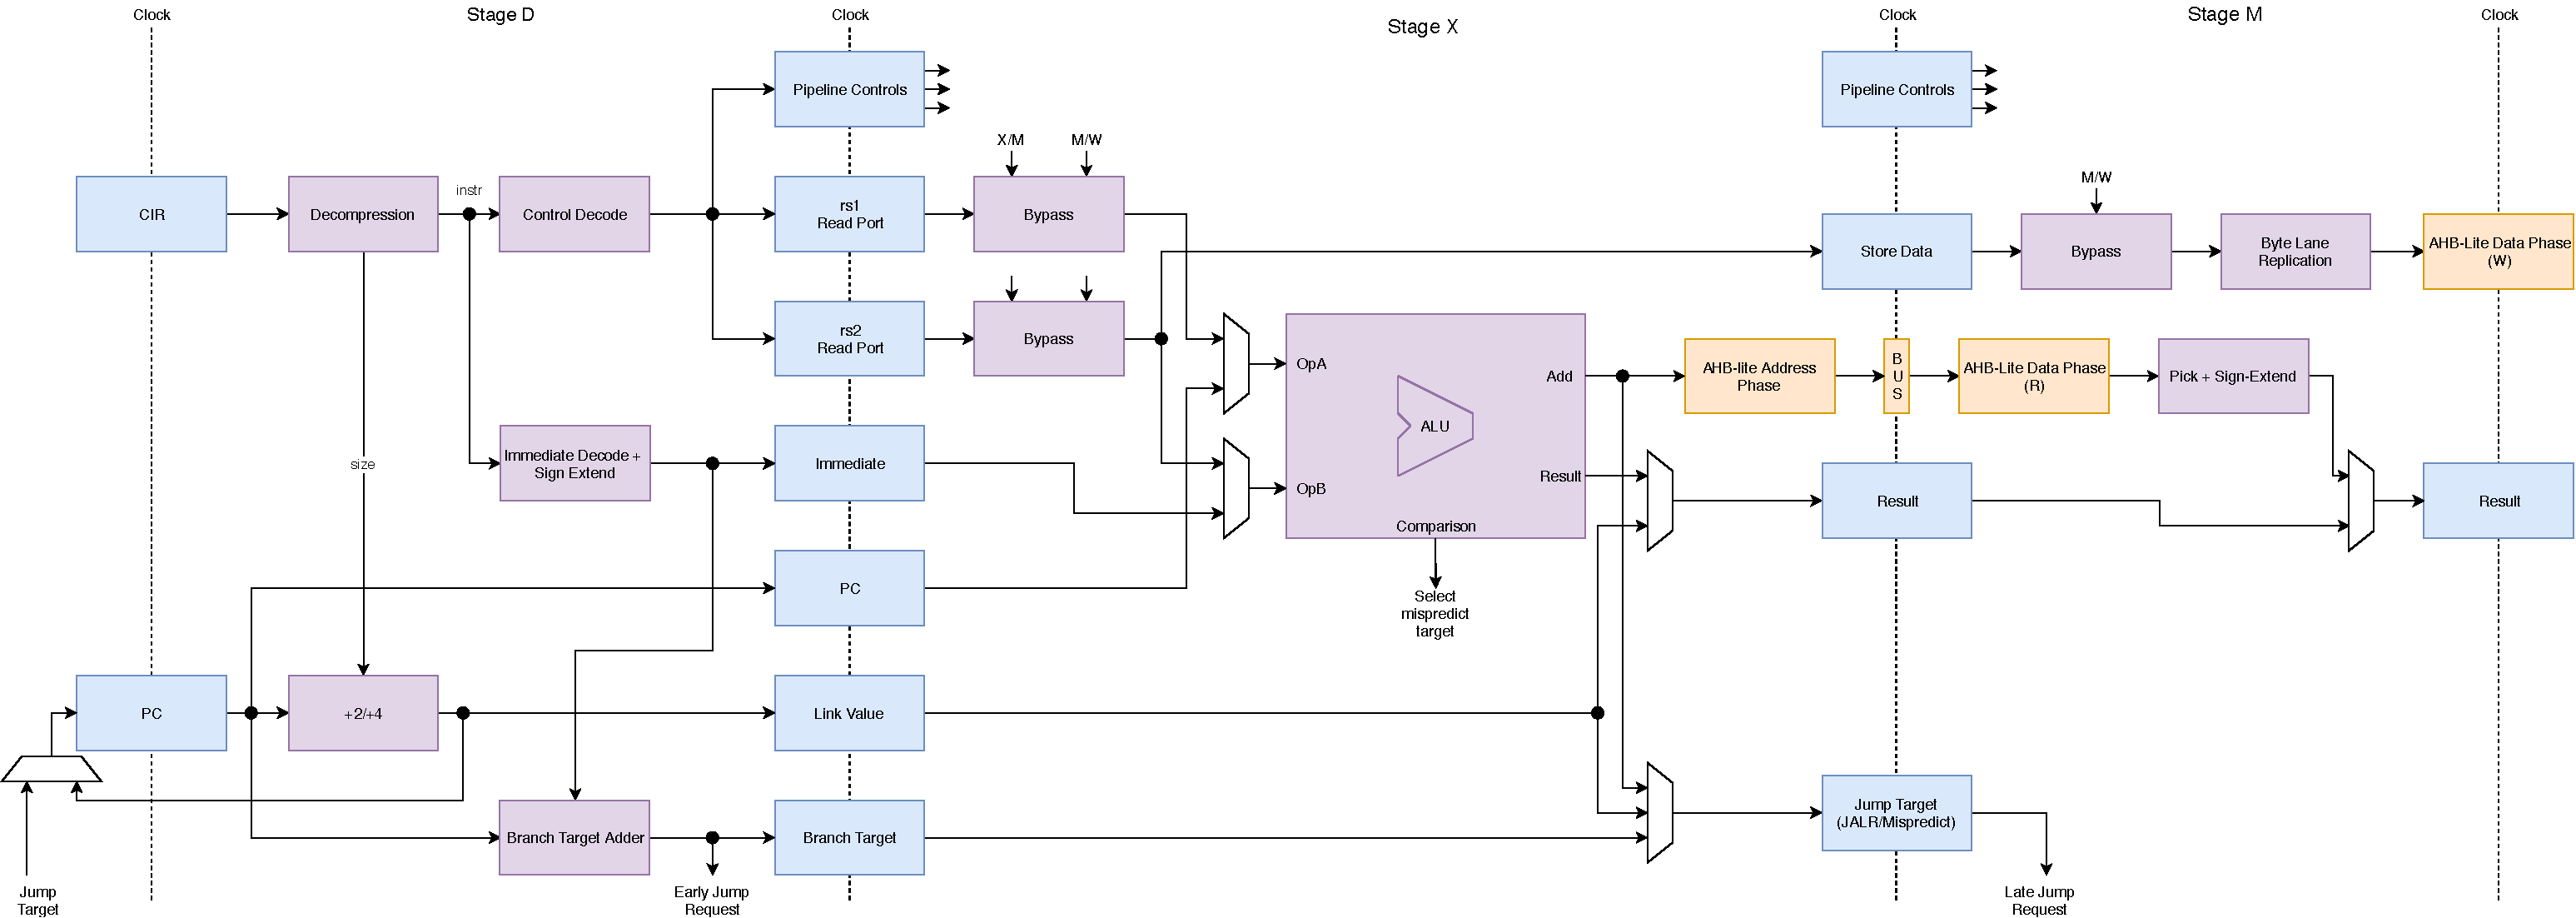
\includegraphics[width=\textheight]{diagrams/cpu_backend.pdf}
			\captionof{figure}{Hazard5 processor backend, block diagram}
			\label{diagram:cpu_backend}
		\end{minipage}
	\end{sideways}
\end{center}

\newpage


\subsubsection{Operand Bypass}

Hazard5 possesses an operand bypass (forwarding) network. Register writes must always be visible to later instructions, even before an earlier instruction reaches register writeback. One solution is to detect that one instruction depends on the result of an earlier instruction (a read-after-write, or RAW hazard) and stall the later instruction until the earlier one completes. This is safe, but incurs a hefty performance penalty; a more elegant solution is to pluck the result of the earlier instruction straight from the pipeline, before it finishes executing (but after the result is valid!).

Locations of bypasses are shown in figure \ref{diagram:cpu_backend}. The following bypasses are available:

\begin{itemize}
	\item {\tt X/M} $\to$ {\tt X}
	\item {\tt M/W} $\to$ {\tt X}
	\item {\tt M/W} $\to$ {\tt M}
	\item {\tt W/X} $\to$ {\tt X}
\end{itemize}

The last is in lieu of a write-to-read bypass in the register file; some tools (not Yosys!) struggle with inferring memories from transparent memory models, so it's better to be explicit.

To control the bypassing, some of the register specifiers from {\tt CIR} are passed down the pipeline alongside the data. {\tt rs1, rs2, rd} (operand sources and destination) are passed down as far as {\tt X}. {\tt rs2, rd} make it to {\tt M}, and only {\tt rd} makes it to {\tt W}.

The upshot is:

\begin{itemize}
	\item Back-to-back ALU operations execute at 1 CPI
	\item Loads insert 1 stall cycle if immediately required by the ALU. 1 CPI otherwise.
	\item Stores execute at 1 CPI (bus stall notwithstanding)
	\item In a load + store pair, the load takes only one cycle, since the {\tt M} stage has self-forwarding
\end{itemize}

Various interesting strategies can alleviate load-use penalty in in-order pipelines, such as adding a second, "late" ALU in the {\tt M} stage. In our case we judge this to not be worth the LUTs.

Another interesting strategy is to add muxing at the register file write port, to select which stage to retire from. This has the dual benefit of firstly simplifying the operand bypass, and secondly reducing dynamic power, since there is no need to pass data through unused stages (and they can be clock gated). Hazard5 does not use this strategy either -- maybe the next project.

\subsubsection{Pipeline Stalling and Flushing}
\label{section:stalling_flushing}

Our terminology: stalling means a pipeline stage does not advance its state until some blocking condition has cleared. The instruction residing in this stage will not progress to the next stage, and the previous stage will not write {\it its} instruction into this stage. Flushing is when in-flight instructions in some stages are replaced with NOPs, and their results are discarded.

The frontend is decoupled from other stages' stall logic via the prefetch queue. This is important: {\tt hready} is an input to that stall logic, and the the frontend's address-phase request must not be a function of {\tt hready}.

The frontend may not be able to immediately accept a jump request, which may cause other pipe stages to stall if it is low. One cause is the frontend holding an existing address-phase request stable until the cycle {\it after} {\tt hready}, which is required for AHB-Lite compliance.

For the backend, the stall logic is more intricate, as signals such as {\tt hready} are used in-cycle to determine whether an instruction progresses to the next pipeline stage:

\begin{itemize}
	\item {\tt D}:
	\begin{itemize}
		\item {\tt CIR} does not contain a valid instruction (either no data, or half of a 32-bit instruction)
		\item {\tt D} asserts jump, but frontend rejects the jump request
		\item {\tt X} is stalled
	\end{itemize}
	\item {\tt X}:
	\begin{itemize}
		\item {\tt hready} low and {\tt X} address-phase request asserted
		\item RAW hazard on {\tt M} (load-use)
		\item {\tt M} is stalled
	\end{itemize}
	\item {\tt M}:
	\begin{itemize}
		\item {\tt hready} low and data-phase active
		\item {\tt M} asserts jump, but frontend rejects the jump request
	\end{itemize}
	\item {\tt W}: does not stall
\end{itemize}

If a given stage is stalled, but the following stage is not, it must insert a bubble. Bubbles are created by zeroing out control fields, such as {\tt rd}, so that the instruction cannot affect system or processor state.

There are two cases where we must flush:

\begin{itemize}
	\item Branch/jump taken from {\tt D}; frontend invalidates prefetched data
	\item Jump/mispredict taken from {\tt M}; must flush frontend, {\tt D}, {\tt X}
\end{itemize}

And the flushing mechanisms for each stage are as follows:
\begin{itemize}
	\item {\tt D}: destination register {\tt rd} cleared, which makes result invisible to register file and operand bypass. {\tt memop}, {\tt branchcond} pipe flags are cleared.
	\item {\tt X}: same as {\tt D} (except for {\tt branchcond}, which does not pass on to {\tt M} anyway.
\end{itemize}

Flushing and bubble insertion are very similar in mechanism.

\subsection{Unaligned Memory Accesses}

Alignment is the constraint that the address of a memory access be equal to zero, modulo some size. Where no size is specified, we refer to {\it natural} alignment, i.e. modulo the size of this particular memory operation. RISC-V requires that memory is byte-addressable.

The frontend goes to some length (section \ref{section:frontend}) to maintain high throughput. RV-C instruction streams are {\it always} unaligned, and {\it every} instruction must be fetched before it is executed, so Amdahl says it's worth it. On the other hand load/stores are less than 100\% of all instructions, and the vast majority are unaligned; consequently, Hazard5 does not have hardware support for unaligned load/stores. These are trapped (TODO) and handled in software if and when they occur.

\subsection{Control and Status Registers (CSRs)}

Hazard5 possesses the standard {\tt Zicsr} extension, which provides atomic access to the CSRs. Only M-mode CSRs are implemented. Access to an unimplemented CSR (e.g. a U-mode or S-mode CSR) causes an illegal instruction exception. The implementation is minimally legal: WARL fields are widely exploited, to reduce logic and state overhead. Module parameters can reduce CSR support, or remove it entirely, as per relative importance of compliance versus area in your application. Note that some features, such as interrupts and exceptions, require CSR support.

When the counter CSRs are present, {\tt mtime} and {\tt mcycle} are aliased to the same counter. 64-bit counters are prohibitively large in a compact 32-bit processor. The {\tt mcountinhibit} (WARL) register is tied to zero: {\tt mtime} must run freely, hence the {\tt mcycle} alias of this counter cannot be halted either. {\tt minstret} is fully implemented, but its {\tt mcountinhibit} bit is also tied low. The width of the counters can be reduced from 64 bits to save logic ({\it noncompliant}), although the full 64 CSR bits remain writeable, which leaves some opportunity for software emulation.

TODO: full table of CSRs we implement, and to what extent they are implemented/WARL'd

\subsection{Interrupts and Exceptions}

Hazard5 has simple exception and interrupt support, compliant with the RISC-V privileged ISA spec (M-mode only). Here we follow the terminology set out in the RISC-V user-level spec: an {\it exception} is an anomalous condition caused by executing an instruction, which requires control transfer; an {\it interrupt} request is some external, asynchronous event, which requires control transfer; a {\it trap} is the transfer of control to a handler, used to service either an interrupt or an exception. Hazard5 implements interrupts and exceptions as follows:

\begin{itemize}
	\item Trap entry causes a jump to a location in the trap vector table (addressed by {\tt mtvec}), simultaneously stashing the PC in {\tt mepc}
	\begin{itemize}
		\item Other CSR state is also modified, e.g. {\tt mcause}, {\tt mstatus}
		\item The physical mechanism for this jump is the same as a branch mispredict
	\end{itemize}
	\item Trap exit, via the {\tt mret} instruction, causes a jump to {\tt mepc}
	\begin{itemize}
		\item {\tt mret} also modifies some diagnostic CSR state, e.g. {\tt mstatus}, as per the privileged ISA specification
	\end{itemize}
	\item Only vectored mode is available. I.e., the LSBs of {\tt mtvec} are tied to 0x1.
	\item When written, {\tt mtvec} is rounded down to a 4kB boundary. This saves an adder when generating the trap vector address.
	\item Besides PC, the hardware saves/restores no architectural state on entry/exit. Software is responsible for stacking/unstacking the GPRs.
\end{itemize}

A custom M-mode CSR {\tt mimsk0} is provided for masking interrupt requests (IRQs):

\begin{itemize}
	\item {\tt mimsk0} is located at address 0xbc0. Addresses 0xbc1...0xbc7 are reserved for more interrupt masks, for $>32$ interrupts.
	\item One bit is provided per external IRQ. 1 = enabled, 0 = disabled
	\item All bits are 0 at reset
	\item Each IRQ has its own slot in the vector table
\end{itemize}

Trap handlers do not preempt one another. After a trap returns, the highest-priority active trap request is selected, and its handler entered. Normal execution continues while there are no active trap requests. Exceptions take priority over IRQs, and lower-numbered IRQs are higher priority. An illegal instruction exception encountered while handling an exception causes a lockup of the core (details TBD). TODO: table of the exception/interrupt space

IRQ inputs are level-sensitive. It is recommended to clear an interrupt at its source upon entering its handler. If the interrupt reasserts before the handler {\tt mret}s, the handler still returns, and the interrupt competes with other trap requests for reentry. Note that, if many register stages are present on the IRQ signal, there is a potential race between clearing the IRQ and executing the {\tt mret}, causing spurious reentry; in practice, restoration of caller-saves should provide ample time for IRQ deassertion to be observed, before the {\tt mret} is reached.


\subsection{Plugin Interface}

Plugins are pieces of hardware attached to the Hazard5 pipeline to extend its functionality, and instruction set. For example, the M extension (multiply and divide) is implemented using a plugin.

Plugins interact with three pipe stages:

\begin{itemize}
	\item {\tt D}
	\begin{itemize}
		\item Plugins see the current instruction, so that they can decode it
		\item Plugins notify {\tt D} that an instruction it does not recognise is, in fact, valid
	\end{itemize}
	\item {\tt X}
	\begin{itemize}
		\item Plugins can see the {\tt rs1} and {\tt rs2} operand bypasses
		\item Additional control signals provide functionality such as killing an in-progress operation so that e.g. an interrupt can run
	\end{itemize}
	\item {\tt M}
	\begin{itemize}
		\item All plugins retire their results into {\tt M}.
		\item This adds a 1-cycle RAW stall if the immediately-following instruction is dependent, but on current iCE40 implementations, {\tt X} is already near-critical-path and very mux heavy.
		\item Plugins can stall {\tt M} if they need more cycles to produce a result.
	\end{itemize}
\end{itemize}

There is no hard limit to the number of plugins that can be added, but the additional muxing and fanout is not free, which constrains practical implementations.

\subsubsection{M-small Plugin}

The M-small plugin implements the RISC-V M standard extension (multiply, divide and modulo). To save area, the plugin employs a combined multiply/divide unit which performs all required calculations, at 1 bit per clock. If timing permits, the datapath can be unrolled to perform multiple iterations per clock. e.g. radix-4 divide/multiply.

\subsubsection{M-fast Plugin}

The Mfast plugin also implements the M extension, but uses a fast Wallace tree to perform multiplication, allowing a throughput of 1 32-bit multiply per clock.

Other details TBD
